\documentclass[10pt,twocolumn,prl,aps,floatfix,superscriptaddress,longbibliography]{revtex4-1}

\usepackage{pdfpages} % include pdfs
\usepackage{pgffor} % for loops

% This deals with a pdfpages rotation bug with revtex
\makeatletter
\AtBeginDocument{\let\LS@rot\@undefined}
\makeatother

\begin{document}

\title{Combining supplemental material into your manuscript as a separate pdf
file suitable for posting to the arXiv}

\author{Adrian Del Maestro}
\email{Adrian.DelMaestro@uvm.edu}
\affiliation{Department of Physics, University of Vermont, Burlington, VT 05405, USA}
\affiliation{Institut f\"ur Theoretische Physik, Universit\"at Leipzig, D-04103, Leipzig, Germany}

\begin{abstract}
    Here I describe a convenient method for managing manuscript and supplemental
    material files separately, then easily combining them for submission to
    journals or the arXiv while using a common bibtex bibliography file.
\end{abstract}
\maketitle

% ---------------------------------------------------------------------------------
% Introduction
% ---------------------------------------------------------------------------------
Journals often require that supplemental material be uploaded as a
self-contained \texttt{.pdf} file while an arXiv submission needs all material to be
included in a single \texttt{.tex} file.  This can cause problems when using
bibtex, especially if the same references are cited in both the manuscript and supplement.
Here I present a solution to this problem based on an answer posted on
\LaTeX~Stack Exchange \cite{tex} that I have recently used in two arXiv
posting \cite{Sengupta:2017tl, Barghathi:2018rg}.

The header of the main manuscript file should include the following packages
and code:
%
\begin{verbatim}

\usepackage{pdfpages} % include pdfs
\usepackage{pgffor}   % for loops

% A fix for revtex-pdfpages rotation bug 
\makeatletter
\AtBeginDocument{\let\LS@rot\@undefined}
\makeatother
\end{verbatim}
%
where \texttt{pdfpages} facilitates the inclusion of external multi-page PDF
files in \LaTeX~documents \cite{pdfpages} and \texttt{pgffor} allows one
to write simple for loops.  The bug fix for dealing with page rotation was
found here \cite{rotate}.

After generating the appropriate \texttt{supplement.pdf} with $N$ pages using a
separate latex file, one can then include it at the end of the manuscript
(after \texttt{\textbackslash bibliography\{refs\}} but before \texttt{\textbackslash end\{document\}}) via the
following code:
%
\begin{verbatim}
\foreach \x in {1,...,N} 
{
\clearpage
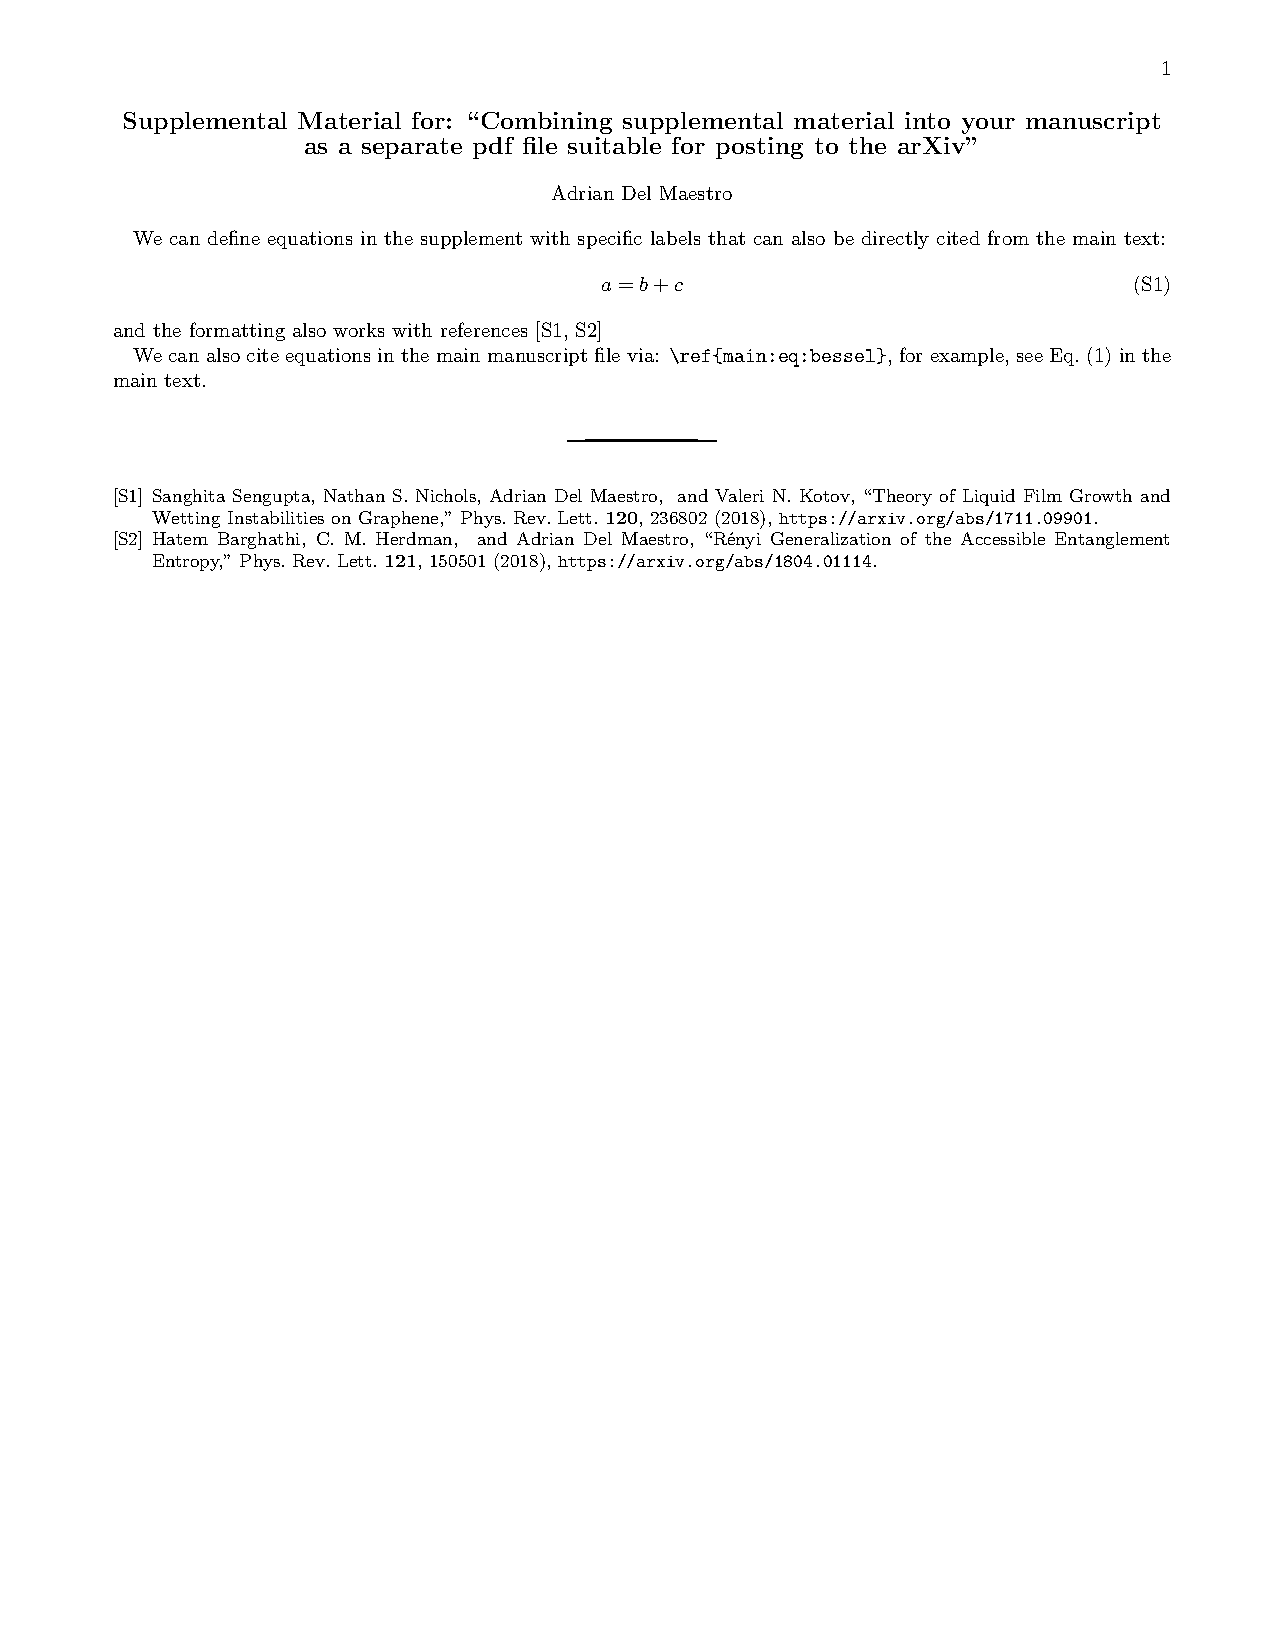
\includepdf[pages={\x,{}}]{supplement.pdf}
}
\end{verbatim}
%
where $N$ should be replaced with the number of pages in your PDF file.   See
the included \texttt{supplement.tex} file for details on how to add unique
labels to equation and references.

The arXiv submission should include \texttt{manuscript.tex},
(\texttt{manuscript.bbl} if using \texttt{bibtex}) and
\texttt{supplement.pdf} while for the journal submission, you can simply
comment out the above block of code in the manuscript file. 

\bibliography{refs}


\foreach \x in {1,...,2}
{
\clearpage
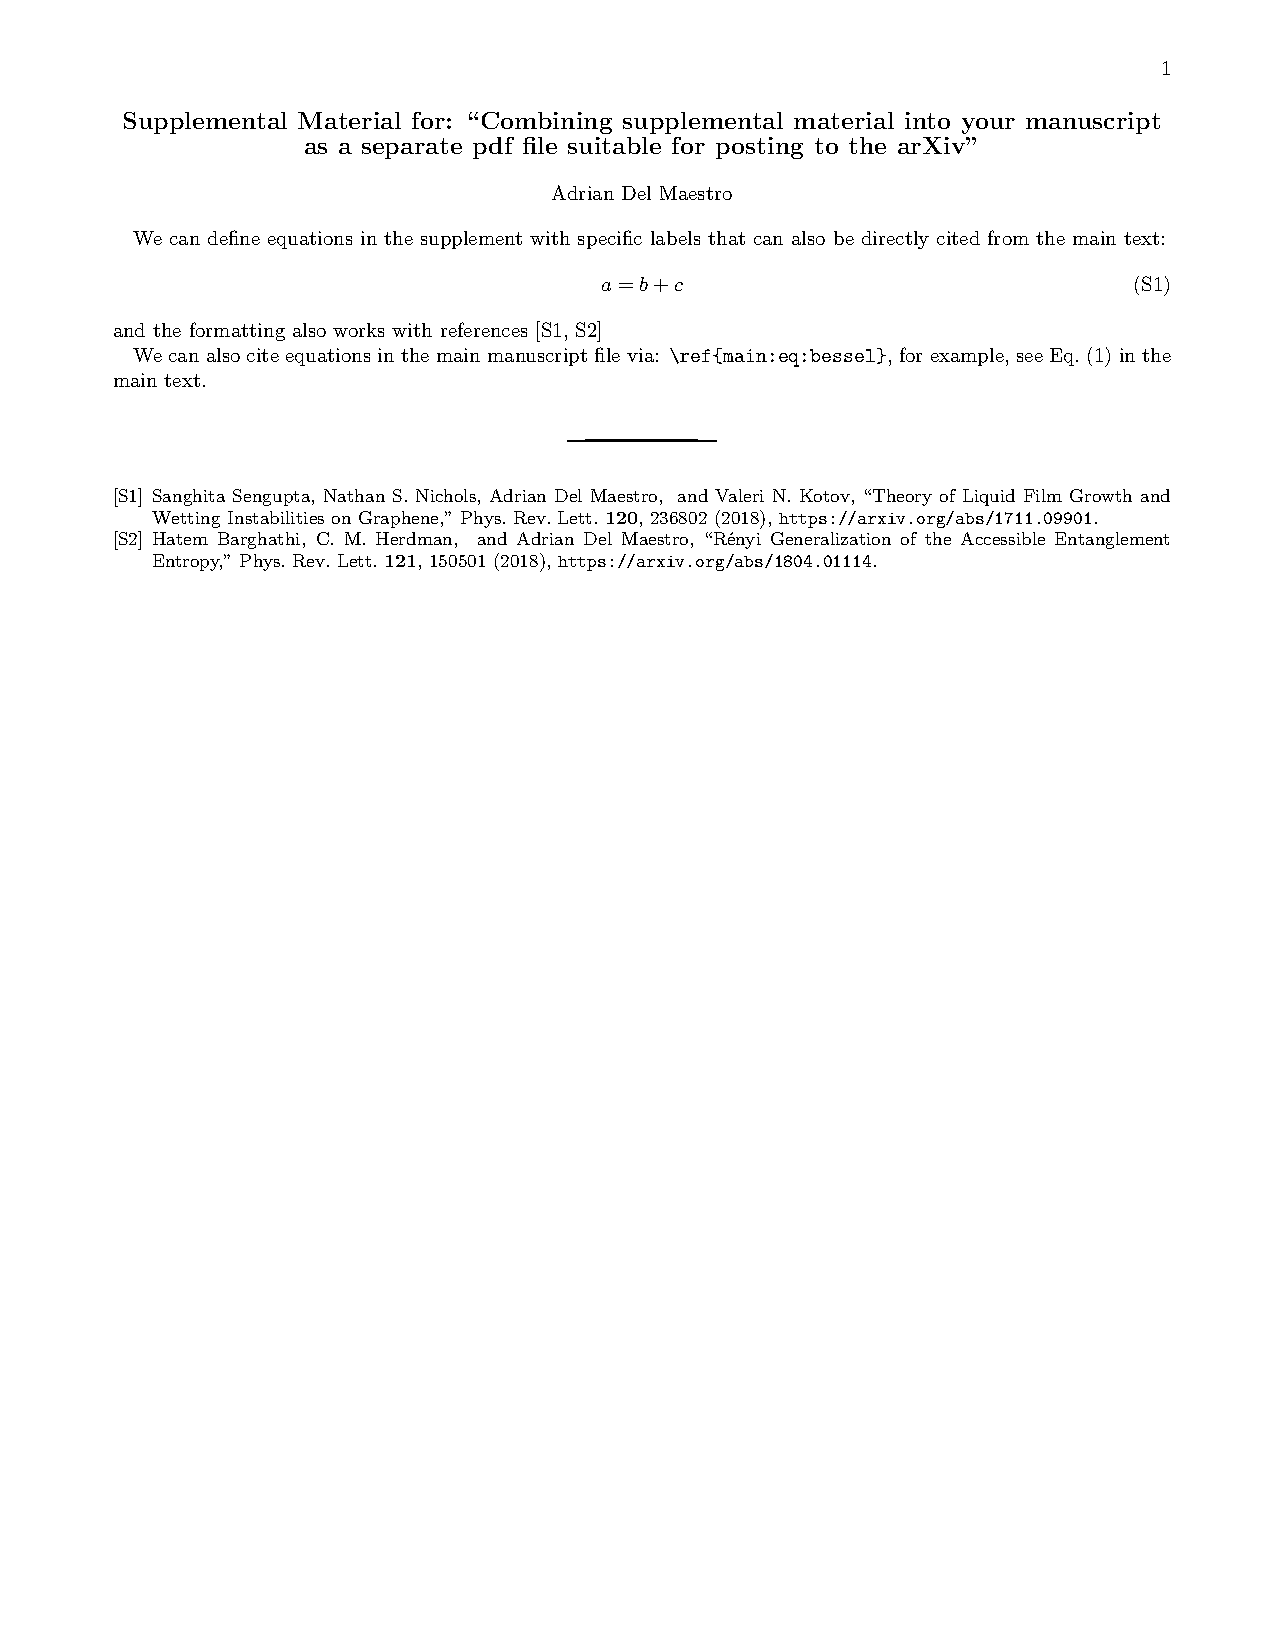
\includepdf[pages={\x,{}}]{supplement.pdf}
}

\end{document}
